%
% $RCSfile: biological_reflections.tex,v $
%
% Copyright (c) 2001-2004. Christian Heller. All rights reserved.
%
% No copying, altering, distribution or any other actions concerning this
% document, except after explicit permission by the author!
% At some later point in time, this document is planned to be put under
% the GNU FDL license. For now, _everything_ is _restricted_ by the author.
%
% http://www.cybop.net
% - Cybernetics Oriented Programming -
%
% http://www.resmedicinae.org
% - Information in Medicine -
%
% @author Christian Heller <christian.heller@tuxtax.de>
%

\section{Biological Reflections}
\label{biological_reflections_heading}

The previous sections have shown how existing patterns for communication can be
merged into one common system architecture. All of these design patterns suggest
their very own communication paradigm which cannot be used anymore in the new,
merged \emph{Translator} architecture. Therefore, a new way for system interaction
needs to be found.

\begin{figure}[ht]
    \begin{center}
        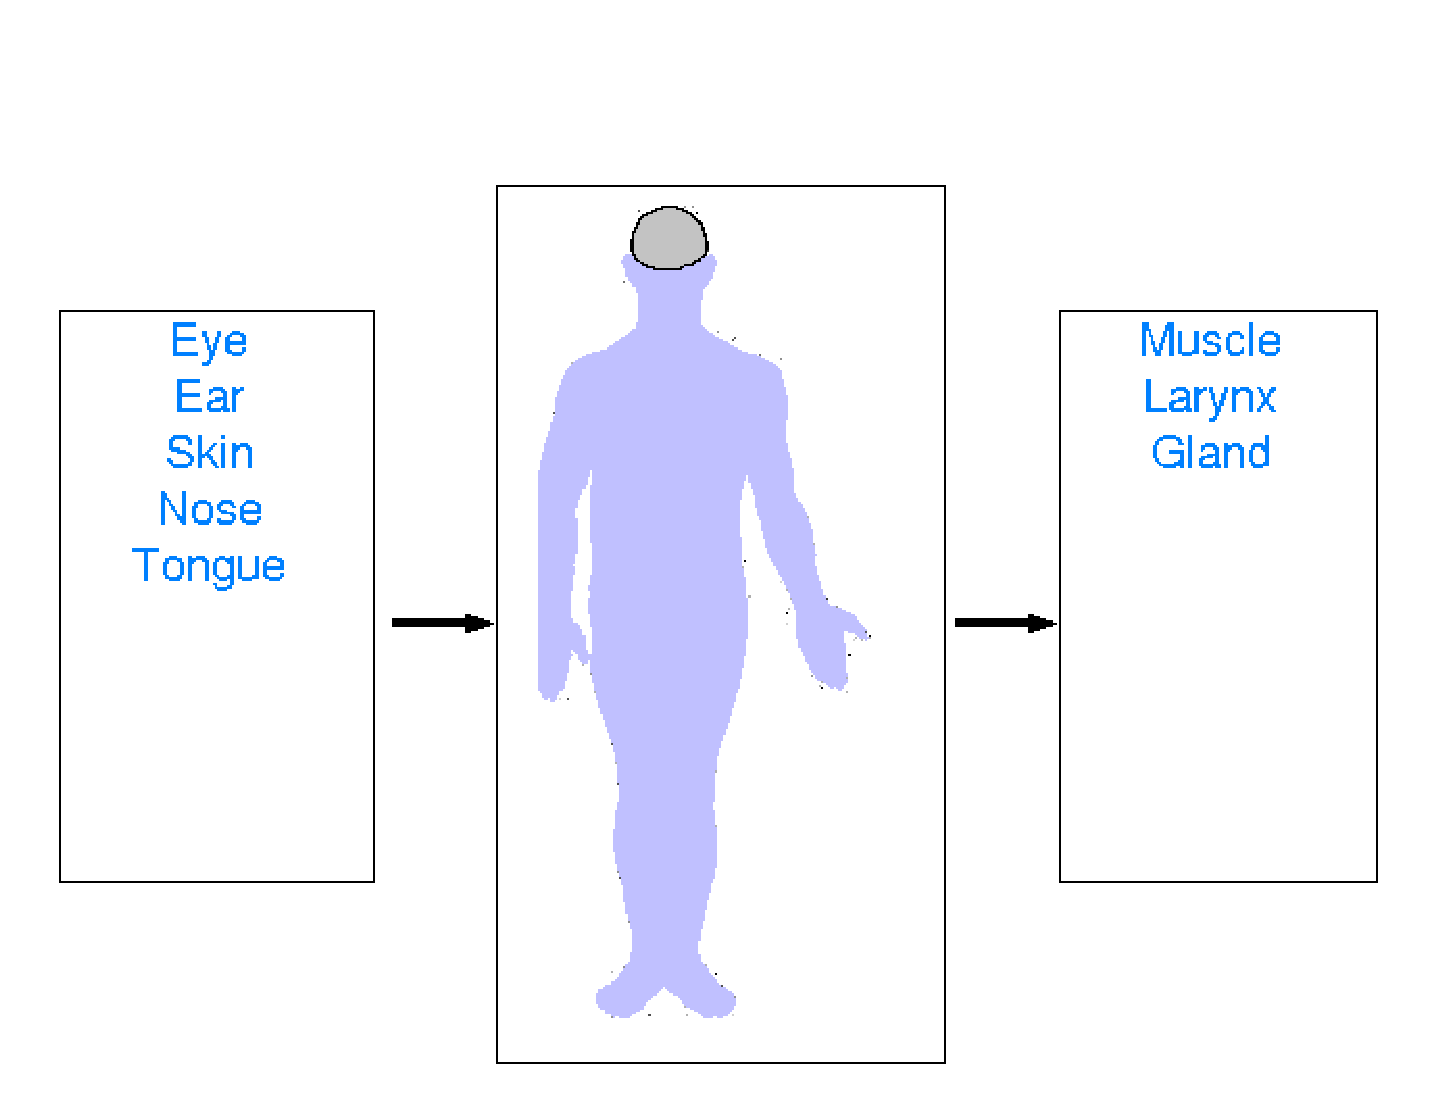
\includegraphics[scale=0.3]{vector/human_being_as_system.eps}
        \caption{Human Being as System of Models (Brain)}
        \label{human_being_as_system_figure}
    \end{center}
\end{figure}

Following the CYBOP approach, nature -- in our case the Human body -- will be
considered next. Humans have organs responsible for information input and output
(figure \ref{human_being_as_system_figure}). In between input and output, the
information is processed by the brain that contains a specific abstract model
of the surrounding real world. The human brain consists of several regions, each
being responsible for a special task, such as the optical region for seeing or the
cerebral cortex for actual information processing which possibly leads to awareness.

\begin{figure}[ht]
    \begin{center}
        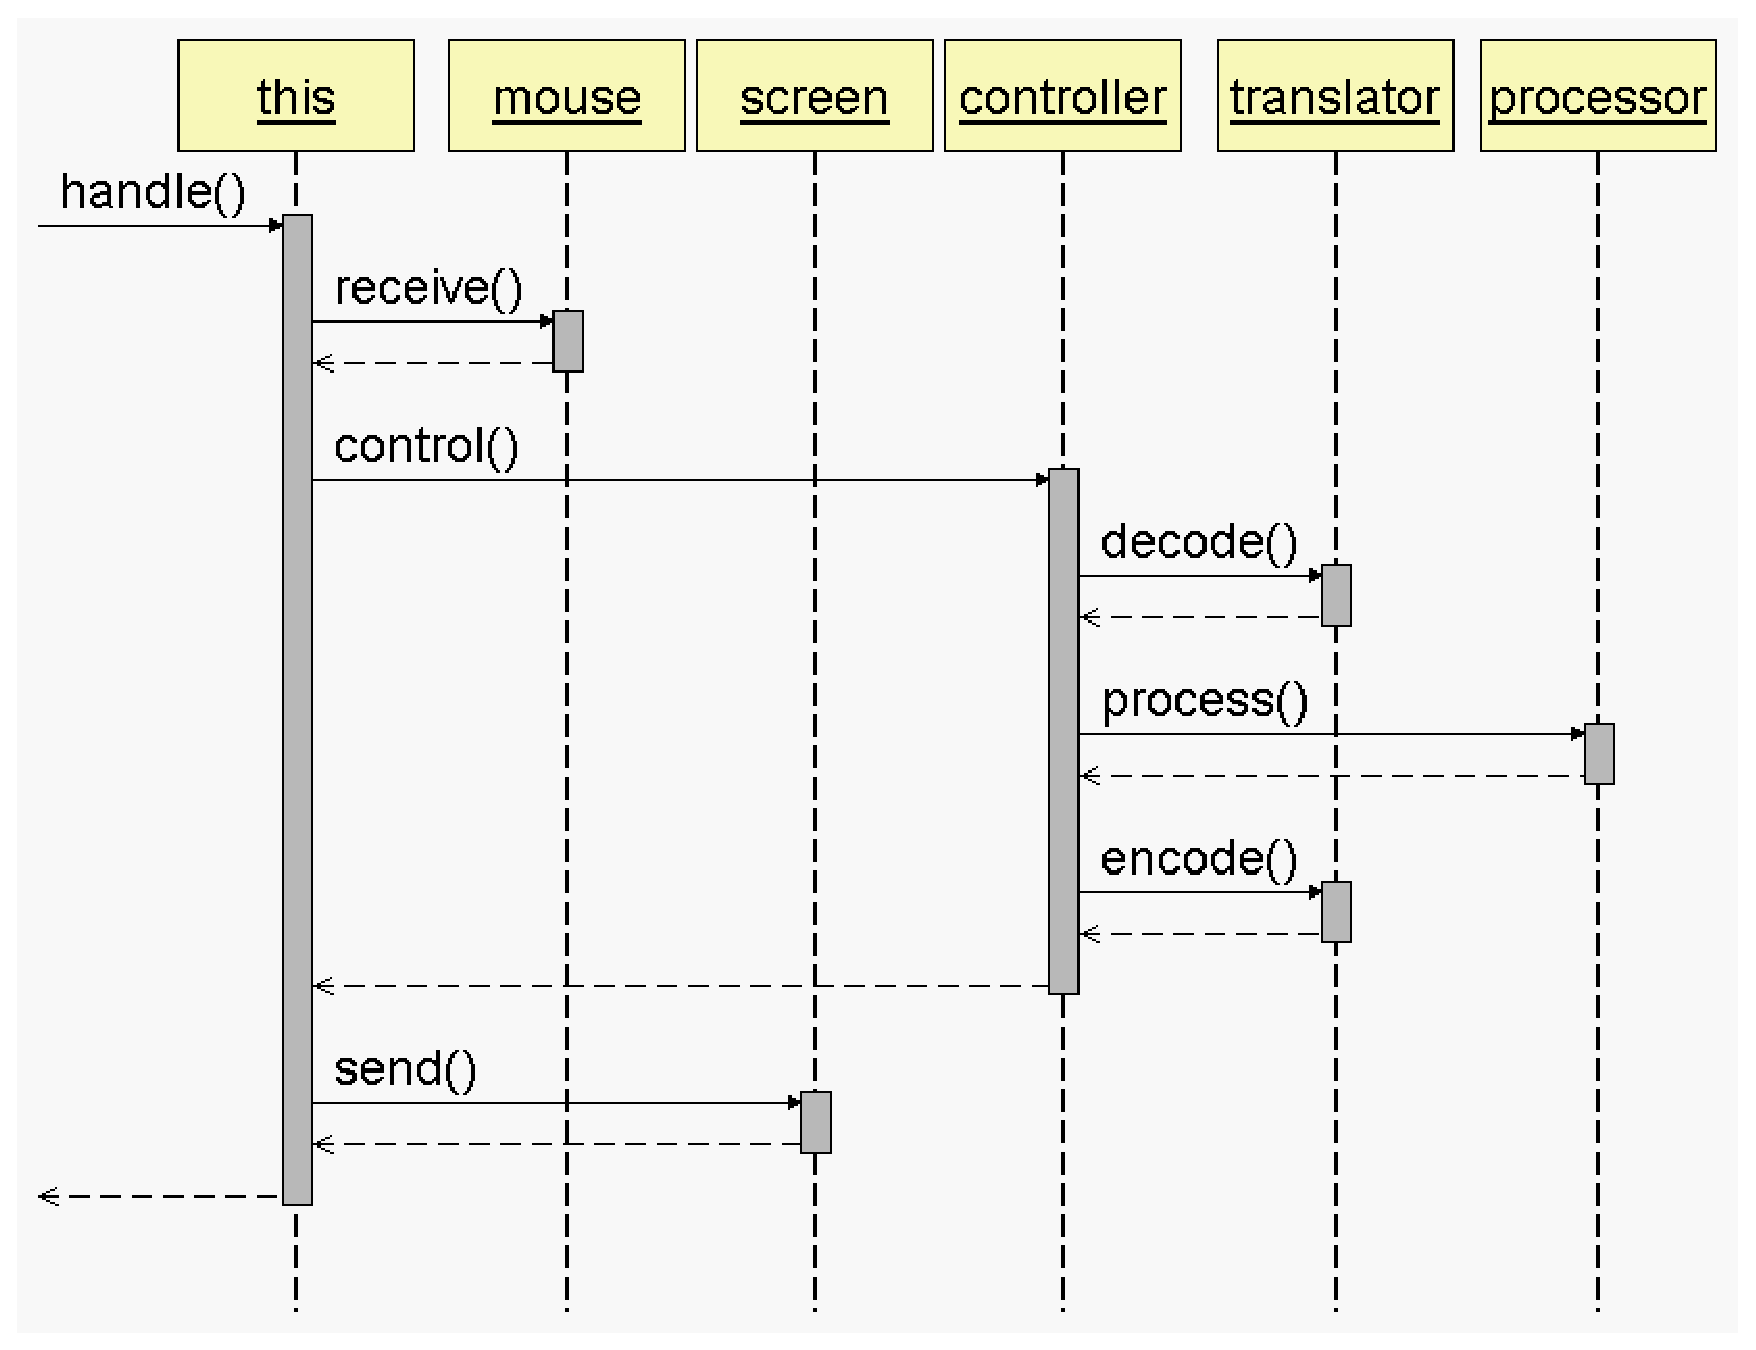
\includegraphics[scale=0.3]{vector/signal_processing.eps}
        \caption{Signal Processing as UML Sequence Diagram}
        \label{signal_processing_figure}
    \end{center}
\end{figure}

The following example demonstrates a typical information (signal) processing
procedure (technical names were used instead of biological ones in figure
\ref{signal_processing_figure}; the terms \emph{Mapper} and \emph{Assembler}
are converted and merged into the term \emph{Translator}):\\
One human \emph{System} wants to send another human \emph{System} a message.
It decides for an acoustical \emph{Signal}, formulates a sentence and talks to
the other human \emph{System} (\emph{handle} method). The other human receives the
\emph{Signal} across its ear organ (\emph{Keyboard}, \emph{Mouse}, \emph{Network}).
The \emph{Signal} is then forwarded to the receiver's brain (\emph{Controller})
where a special \emph{Region} responsible for acoustics (\emph{Translator})
translates (\emph{decode} method) the data (\emph{DataTransferModel}) contained
in the \emph{Signal} and sorts them into the human's abstract model of the
surrounding real world (\emph{DomainModel} or \emph{KnowledgeModel}, respectively).
Processing of the signal happens in the cerebral cortex of the brain (\emph{Processor}).
If the addressed listener wants to send an answer \emph{Signal}, it may do so by
triggering a muscle reaction. For this to happen, the motoric brain region (\emph{Translator})
needs to translate (\emph{encode} method) abstract model data (\emph{DomainModel})
into a special communication model (\emph{UserInterfaceModel}) for the answer signal.
Finally, the answer signal will be sent as muscle action (data display on \emph{Screen}).

